\documentclass{article}

% Language setting
% Replace `english' with e.g. `spanish' to change the document language
\usepackage[english]{babel}
\usepackage[affil-it]{authblk}
\usepackage[utf8]{inputenc}


% Set page size and margins
% Replace `letterpaper' with`a4paper' for UK/EU standard size
\usepackage[letterpaper,top=2cm,bottom=2cm,left=3cm,right=3cm,marginparwidth=1.75cm]{geometry}

% Useful packages
\usepackage{amsmath}
\usepackage{graphicx}
\usepackage[colorlinks=true, allcolors=blue]{hyperref}

\title{The Impact of Offshoring to Mainland China on Taiwan’s Labor Market}
\author{Tung-Sheng Hsieh, supervised by Prof. Hong Ma}
\affil{SEM, Tsinghua University}
\date{May 17, 2019} 

\begin{document}
\maketitle

\begin{abstract}
China’s economic reform in the 1980s and Taiwan’s relaxing of foreign direct investment (FDI) to China has set off a boom for Taiwanese merchants to “go western” to China for offshoring. Low-skilled labors in the home economy are predicted by economic theory to be adversely impacted by the offshoring activity, and data shows a trend of decreasing low- skilled labor demand in Taiwan accompanying with the rising FDI to and imports from China. This paper studies the adverse impact of offshoring on low-skilled labor in Taiwan’s 23 manufacturing industries from 2003 to 2017 and tailors the measure of offshoring according to its attributes of investment in China. The sign of the coefficient estimates of offshoring using the tailored measurement contradicts with the prediction of offshoring theory possibly due to the reverse causation. Instrumental variables depicting the ex-ante situation of each industry were introduced to control for the impact of skilled-biased technological change (SBTC) but failed to pass the validity test. Coefficients estimates based on three offshoring indexes implied by Jensen and Kletzer (2005) ~\cite{jensen2005tradable}are all insignificant.\\

\textbf{Keywords}: Offshoring; Foreign Direct Investment; Low-skilled labors; China; Taiwan

\end{abstract}

\section{Introduction}

More than twenty years have passed since the establishment of the World Trade Organization, the largest trade community in human history and the most recognized icon of the globalization. Multinational firms stretch their production network and specialize in different production process globally to yield the production benefit. Although the reallocation of work increases the firm’s productivity, its effect on the labors in the home country is not always positive. Hsieh and Woo (2005)~\cite{hsieh2005impact} suggest empirically that Hong Kong’s low-skilled labor had been adversely impacted in terms of wages and employment since the start of massive outsourcing to China in the 1980s. Like Hong Kong, Taiwan is an Asian newly industrialized economy trading frequently with and invest heavily in China since then. As shown in Figure 1, Taiwan has experienced emerging foreign direct investment to and a huge volume of import from China since 1991, one year after the Taiwan government relaxing of regulations on investment to mainland China.\par 
\begin{figure}
\centering
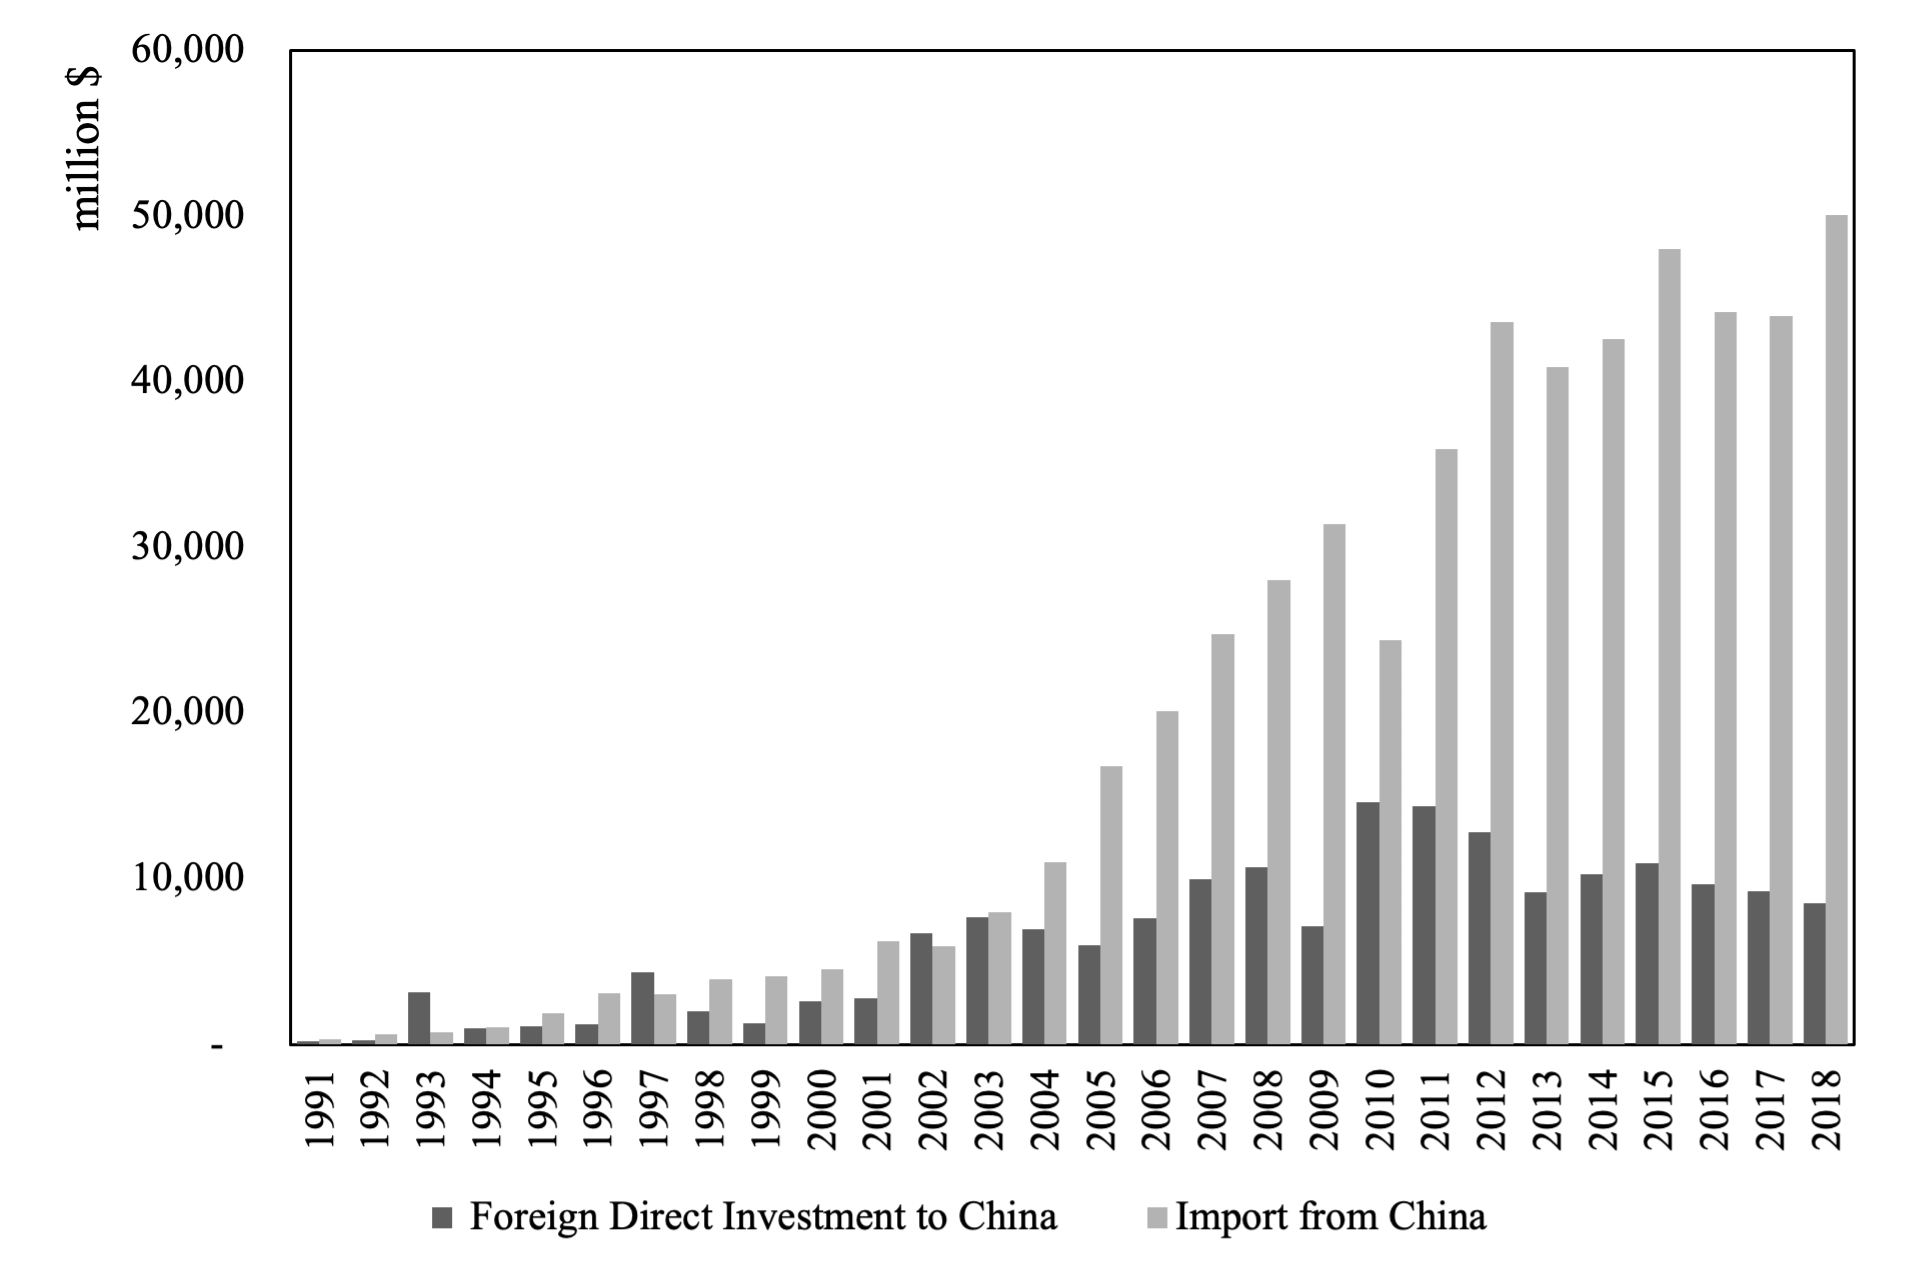
\includegraphics[width=1\textwidth]{figure1.png}
\caption{\label{fig:1}Taiwan's Foreign Direct Investment to and Import from China, 1991-2018}
%\source{The Bureau of Foreign Trade; Investment Commission, MOEA, Taiwan (ROC)}
\end{figure}
At the same time, as shown in Figure 2, Taiwan has experienced a decrease in the wage-bill share of production workers (i.e., low-skilled workers), which coincides with the implication of the simplest offshoring model. 
\begin{figure}
\centering
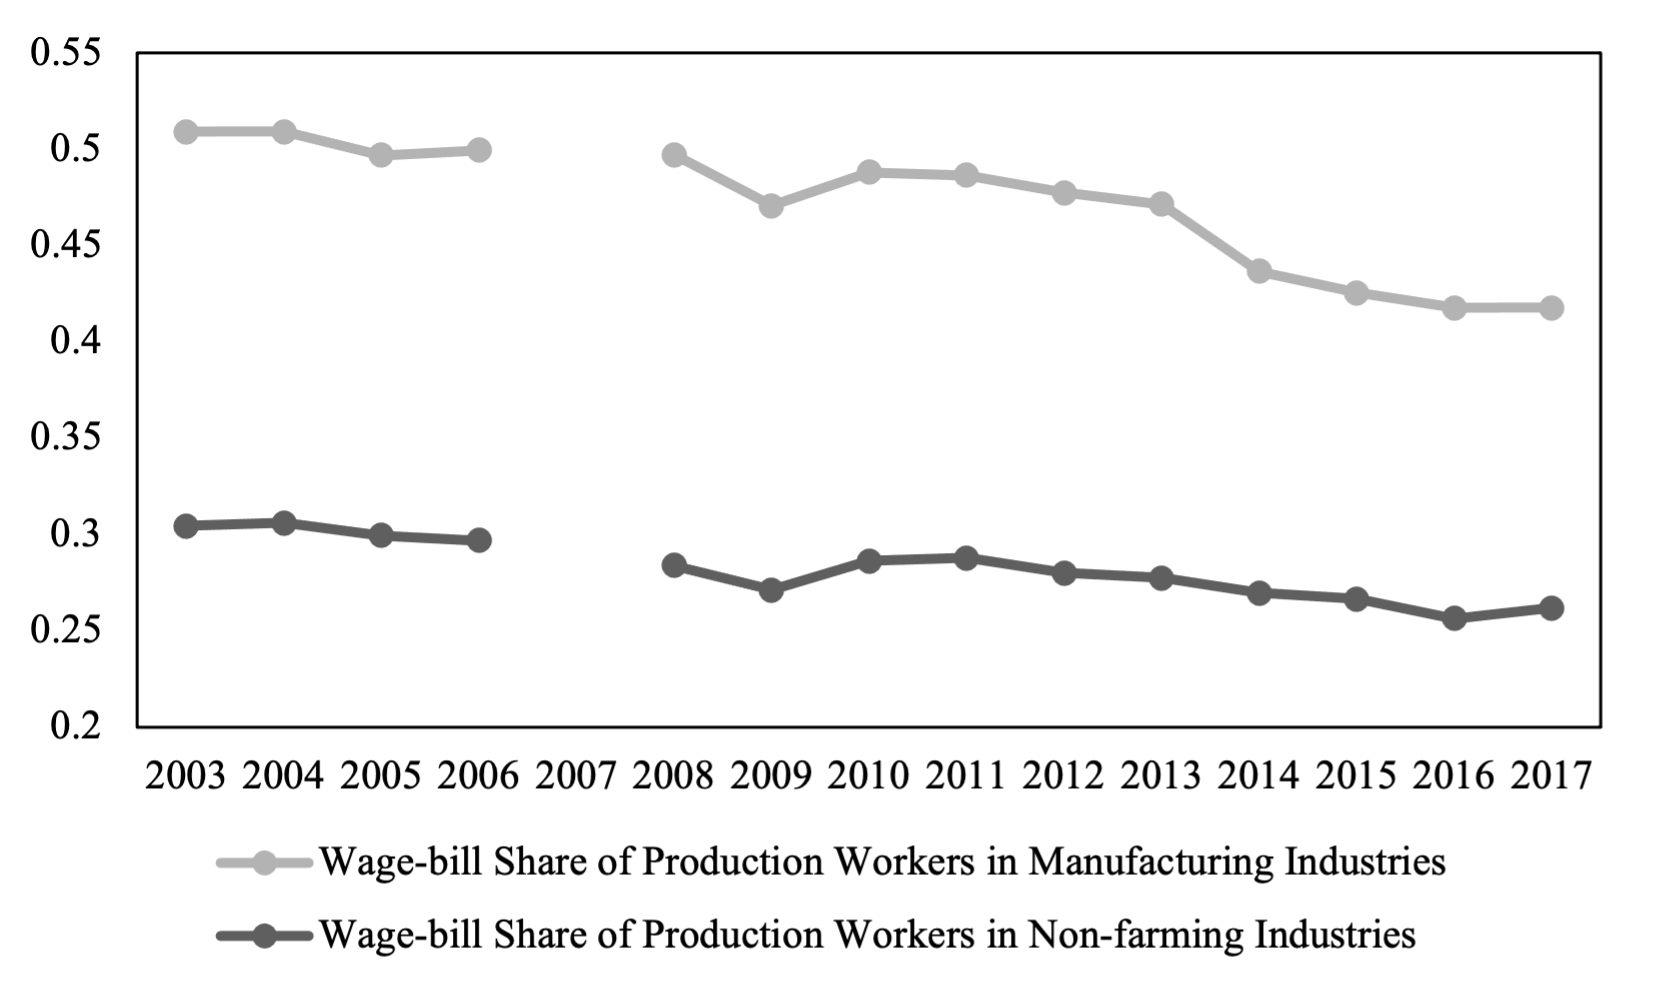
\includegraphics[width=1\textwidth]{figure2.png}
\caption{\label{fig:2}Wage-bill Share of Production Workers in Taiwan, 2003-2017}
%\source{}
\end{figure}
The goal of this paper is to find out the impact of offshoring to China on Taiwan’s low-skilled labor in manufacturing industries and give the implication to policymakers in economies with a comparable size that depends heavily on foreign trade and offshoring. Base on the regression proposed by Hsieh and Woo (2005)~\cite{hsieh2005impact}, we proposed a new measurement of offshoring that better describes the characteristics of Taiwanese foreign direct investment in China. 
The paper proceeds as the following. Chapter 2 discusses the specification of the regression and data selection. Chapter 3 shows the outcomes of the regression analysis, and Chapter 4 concludes.


\section{Data and Regression Specification}

\subsection{Regression Function}

Combining Berman, Bound, and Griliches (1994)~\cite{berman1994changes}, Feenstra and Hanson (1995)~\cite{feenstra1995foreign}, and Hsieh and Woo (2005)~\cite{hsieh2005impact}, we have the following regression function.
$$\Delta D_{t,i}=\beta_1\Delta Off_{t,i}+\beta_2\Delta\ln(K_{t,i}/Y_{t,i})+\beta_3\Delta SBTC_{t,i}+\beta_4 Time_t+\beta_5\ln d_i+\varepsilon_{t,i}$$\par

The dependent variable is the change in the wage-bill share of production workers (low-skilled workers) of different industries $j$ within the manufacturing sector between the year $t$ and $t-1$. On the right-hand side, the independent variable of interest is the change in offshoring in the industry $j$. Here we first follow the measurement of offshoring adopted by Hsieh and Woo (2005)~\cite{hsieh2005impact} using change in share of imports from China as a fraction of imports from China and domestic outputs. However, the validity of this measurement is based on the fact that a huge share of Hong Kong’s import from China is used for the reexport, which may not be in the case of Taiwan. To better measure the offshoring from Taiwan to China, this paper replaces the original index with the change in the foreign direct investment (FDI) from Taiwan to China as a fraction of total domestic output. In addition to the offshoring, the prevalent skilled-biased technological change (SBTC) may also contribute to the change in the demand for low-skilled workers. Here we use change in the employment share of Taiwan’s production workers as the measurement of SBTC and introduce the change in capital-output ratio to control for the capital-skill complementarity. Finally, the paper introduces both time and industry dummies to control for time and industry fixed effects.\par

The descriptions of variables are summarized as follows. $\Delta D_{t,i}$ is the annual change in production worker's share of the wage bill. $Off1_{t,i}$ is the annual change in share of imports from China as a fraction of imports from China and domestic outputs. $Off2_{t,i}$ is the annual change in FDI from Taiwan to China as a fraction of total domestic output. $\Delta \ln (K_{t,i}/Y_{t,i})$ is the annual change in the capital-output ratio. $SBTC_{t,i}$ is the annual change in the employment share of production workers. $Time_t$ is the time dummies for 13 annual differences. $\ln d_i$ is the industry dummies for 23 industries.\par

\subsection{Data Collection and Description}

All the data are from the Taiwan government’s website. The data of wage and employment are from The Ministry of Labor, and the period of the data starts from 2003 to 2017 with 2007 unavailable. This paper gathers data of 23 industries in the manufacturing sector classified under Taiwan’s Standard Industrial Classification (TSIC) Revision 7. Some data of years that classified using newer version are clustered or broken down to map to the original classification. The paper then defines the Elementary Occupations (code:900000) and Plant and Machine Operators and Assemblers (code:700000) under Taiwan’s Standard Occupational Classification System Revision 5 as the production workers. The data of import from China is gathered from the Bureau of Foreign Trade. The paper constructs the outsourcing index for each industry by mapping the six-digit Harmonized Commodity (HS) code of imported goods to the International Standard Industrial Classification (ISIC) and then mapping it again to the 23 industries under TSIC Rev. 7. The paper concords every year’s data to HS 1996 and ISIC Revision 3. The data of FDI from Taiwan to China are gathered from the Investment Commission, MOEA. The capital of 23 industries are collected from the Industry and Service Census conducted by Directorate-General Budget, Accounting and Statistics, Executive Yuan once every five years, so only capital of 2001, 2006, 2011 are available. We then interpolate the capital for other years. Finally, the data of domestic output are from the Department of Statistics, MOEA. The statistics of data observations are summarized in Table 1.

\begin{table}[]
    \centering
    \begin{tabular}{ |cccccc| } 
 \hline
 Variables & Obs & Mean & Std. & Dev. & Min\\
 $D$ & 299 & -0.0037652 & 0.0488521 & -0.3879308 & 0.2303175 \\ 
 $Off1$ & 299 & 0.0189355 & 0.0622801 & -0.5529502 & 0.3110296 \\ 
 $Off2$ & 299 & 2.54e-06 & 0.0018006 & -0.0127272 & 0.0195498 \\ 
 $dlnky$ & 299 & 0.0280908 & 10.98118 & -22.61537 & 25.2704\\
 $SBTC$ & 299 & -0.0031365 & 0.0271699 & -0.2512667 & 0.1020601\\
 \hline
\end{tabular}
    \caption{Summary Statistics of Data Observations}
    \label{tab:1}
\end{table}





\section{Regression Outcomes}
\begin{figure}
\centering
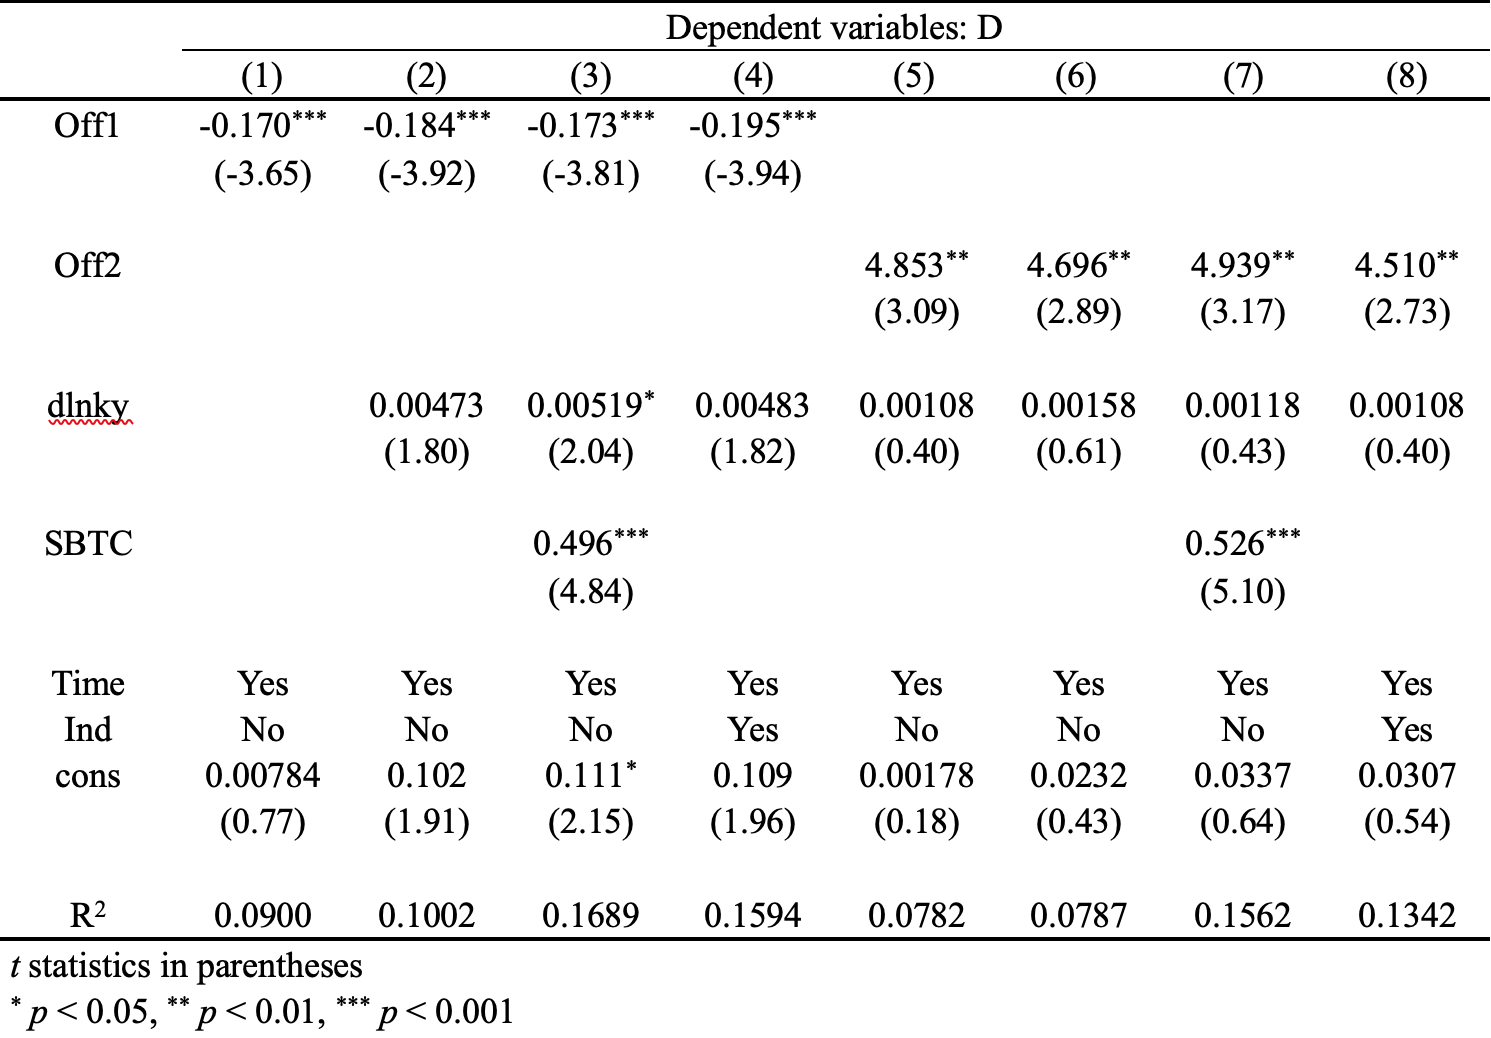
\includegraphics[width=1\textwidth]{Screen Shot 2021-05-24 at 21.56.19.png}
\caption{\label{fig:3}OLS Estimates of Relationship between Offshoring and Demand of low-skilled Labors}
\end{figure}

Table 2 shows the OLS estimates of $\beta$ of the regression illustrated in the previous section. The first column is the result of the baseline regression and, as implied by the offshoring model, has a negative impact on the demand for low-skilled labors. The estimate of the coefficient is significant at 0.001 level and suggest that 1 point increase in the fraction of import divided by the sum of import and domestic output will cause the wage-bill share of low skilled labor to decrease 0.17. The control for changes in the capital-output ratio is introduced in the second column. Although the coefficient for the control variable is not significant at all,$\beta 1$ decreases further to -0.184, still with significance at 0.001 level. In column three, the SBTC was controlled to exclude the effect of skill upgrading. The coefficient of the SBTC is, surprisingly, positive, making $\beta 1$ slightly larger than that in the baseline regression. It is possible that the measurement of SBTC may need to be altered to capture better the change in the technology favoring high-skilled labor. In the fourth column, industry dummies were introduced to control for industry fixed effects. The other half of the table replace the original offshoring measure with the one that better captures the characteristics of the offshoring from Taiwan to China, which is the FDI divided by the domestic output of each industry. However, the sign of the coefficient surprisingly turns positive in all four regressions with significance at 0.01 level, meaning that a point increase in the FDI-output ratio contributes to the increase in 4 to 5 points increase in the wage- bill share of production workers, which may be counterintuitive in this setting. One of the possible and obvious reason may be that there exists some extent of reverse causation. It is possible that the industry which invests more in China is the one with a higher wage-bill share of production workers. To better exclude the endogeneity, the introduction of feasible instrumental variables for the offshoring index will be discussed. At last, we can see that the increase in SBTC also contributes positively to the increase in the wage-bill share of production workers in the second setting.\par

Additionally, according to Jensen and Kletzer (2005)~\cite{jensen2005tradable}, industries with higher tradability have a higher proportion of employees with a college degree and higher wage level. Thus, the paper uses the proportion of employees with a college degree and above and wage level as two alternative measurements of offshoring. However, the coefficient estimates of both measurements are not significant at all. \par

In the following, we introduce the instrumental variables proposed by Hsieh and Woo (2005)~\cite{hsieh2005impact}. According to their paper, offshoring has a larger effect on industries more labor-intensive and more low-skilled labor-intensive. Thus, instead of using the ex-post figure of offshoring, we can also use the ex-ante characteristics of each industry to gauge its potential “offshorability.” Based on the fact, we introduce the labor share and the wage-bill share of nonproduction workers of the year 2003 as two candidate instrumental variables. However, the two measures did not pass the validity test of being instrumental variables. Both instrumental variables are not correlated with the Off1 and Off2.\par


\section{Conslusion}

The paper presents the fact that Taiwan’s FDI to and imports from China has emerged since Taiwan’s government allowed the domestic investment in China in the 1990s after China opened its markets to the world in 1980s. At the same time, the data shows that the demand for low-skilled labor, as measured by the wage-bill share of production workers, in Taiwan’s domestic market has decreased since then parallelly. The paper then examines the impact of offshoring to the demand of low-skilled labor during the period 2003 to 2017 using measures of offshoring proposed by Hsieh and Woo (2005)~\cite{hsieh2005impact}, FDI index constructed by the author that better portrays the characteristics of Taiwan’s offshoring to China, and measurement implied in Jensen and Kletzer (2005)~\cite{jensen2005tradable}. The sign of coefficient estimates using the first measure aligns with that in Hsieh and Woo (2005)~\cite{hsieh2005impact}, but the coefficient estimates using FDI index shows the counterintuitive sign potentially due to the reverse causation. Two instrumental variables based on the same paper were introduced to remediate the contamination of endogeneity, but both instrumental variables did not pass the validity test. This paper provides empirical support to the concern of labors in similar economies about the adverse impact of further integration with the global value chain. However, institution, including labor regulations, must be taken into account when one tries to apply the result outside of the scope of this paper. Further research on better instrumental variables for offshoring can be studied, and offshoring index should be tailored according to the target country’s characteristics of FDI and trade pattern.\par

\bibliographystyle{plain}
\bibliography{references}

\end{document}